\documentclass{article}
\usepackage{graphicx} % Required for inserting images
\usepackage{fullpage, fourier}
\graphicspath{{images}}
\usepackage{wrapfig}
\usepackage{hyperref}
\usepackage[dvipsnames]{xcolor}
\usepackage{amsmath, amssymb, amsfonts}
\usepackage{caption}
\usepackage[most]{tcolorbox}
\usepackage{listings}
\usepackage{float}
\usepackage{epigraph}
\usepackage{verse}

\hypersetup{
    colorlinks=true,
    linkcolor=blue,
    filecolor=magenta,      
    urlcolor=cyan,
    pdftitle={Overleaf Example},
    pdfpagemode=FullScreen,
    }

\title{Time Dilation}
\author{Ernani Raffo}
\date{May 2023}

\begin{document}

\lstdefinestyle{c}{
  language=c,
  backgroundcolor=\color{white},
  commentstyle=\color{Green},
  keywordstyle=\color{blue},
  keywordstyle=[2]\color{magenta},
  numberstyle=\ttfamily\color{gray},
  stringstyle=\color{BrickRed},
  basicstyle=\ttfamily\footnotesize\color{black},
  breakatwhitespace=false,       
  breaklines=true,                 
  captionpos=b,                    
  keepspaces=true,                 
  numbers=left,                    
  numbersep=7pt,                  
  showspaces=false,                
  showstringspaces=false,
  xleftmargin=10pt,
  showtabs=false,                  
  tabsize=2
}

\newtcblisting{clisting}[2][]{
  title=#2, #1,
  fonttitle=\footnotesize\bfseries,
  colframe=black!75,
  colback=white!90,
  listing only,
  listing options={style=c},
  top=-5pt,
  bottom=-5pt,
  enlarge top by=5pt
}

\lstdefinestyle{python}{
  language=python,
  backgroundcolor=\color{white},
  commentstyle=\color{Green},
  keywordstyle=\color{blue},
  keywordstyle=[2]\color{magenta},
  morekeywords={as, None, True, False, self},
  numberstyle=\ttfamily\color{gray},
  stringstyle=\color{BrickRed},
  basicstyle=\ttfamily\footnotesize\color{black},
  breakatwhitespace=false,
  breaklines=true,                 
  captionpos=b,                    
  keepspaces=true,                 
  numbers=left,
  mathescape=true,
  numbersep=7pt,                  
  showspaces=false,                
  showstringspaces=false,
  xleftmargin=10pt,
  showtabs=false,                  
  tabsize=2
}

\newtcblisting{pylisting}[2][]{
  title=#2, #1,
  fonttitle=\footnotesize\bfseries,
  colframe=black!75,
  colback=white,
  listing only,
  listing options={style=python},
  top=-5pt,
  bottom=-5pt,
  enlarge top by=5pt
}

\lstdefinestyle{bash}{
    language=bash,
    basicstyle=\ttfamily\footnotesize\color{black},
    breakatwhitespace=false,
    mathescape=true,
    breaklines=true,
    captionpos=b,
    keepspaces=true,
    showspaces=false,
    showstringspaces=false,
    xleftmargin=-7pt,
    showtabs=false,
    tabsize=2
}

\newtcblisting{bashlisting}[1]{
    title=#1,
    fonttitle=\footnotesize\bfseries,
    colframe=black!75,
    colback=white,
    listing only,
    listing options={style=bash},
    top=-5pt,
    bottom=-5pt,
    enlarge top by=5pt
}

\lstdefinestyle{llvm}{
    language=LLVM,
    basicstyle=\ttfamily\footnotesize\color{black},
    keywordstyle=\color{blue},
    keywordstyle=[2]\color{magenta},
    breakatwhitespace=false,
    mathescape=true,
    breaklines=true,
    captionpos=b,
    keepspaces=true,
    showspaces=false,
    showstringspaces=false,
    xleftmargin=-7pt,
    showtabs=false,
    tabsize=2
}

\newtcblisting{llvmlisting}[1]{
    title=#1,
    fonttitle=\footnotesize\bfseries,
    colframe=black!75,
    colback=white,
    listing only,
    listing options={style=llvm},
    top=-5pt,
    bottom=-5pt,
    enlarge top by=5pt
}

\maketitle

\section{Introduction}
\setlength{\epigraphwidth}{0.30\textwidth}
\epigraph{\emph{As a basketball around a hoop.}}{--Romilly}
Time dilation is the effect of time moving at a different rate compared to an observer located elsewhere. 
The observers could be in different gravitational fields, or moving at different rates through space.
These differences can play a significant role in their experiences, and is a major plot point of the movie
\textit{Interstellar} directed by Christopher Nolan.
The critically acclaimed movie featured shots in space that were only made possible after hours and hours
of rendering, with highly accurate scientific basis. This is thanks to theoretical physicist Kip Thorne
(\ref{kip}).

\begin{wrapfigure}{r}{0.25\textwidth}

\includegraphics[scale=0.5]{thorne}
\caption{Kip Thorne}
\label{kip}
\end{wrapfigure}

In the movie, the main character, Cooper, goes into space to find a more suitable place for mankind with his space-crew. 
The issue is that one of the most prominent data from exoplanets outside their solar system reside in a system where a 
super massive black hole, Gargantua, sits on the manifold of space-time at a solar mass of 100,000,000. 
The exoplanet, Miller's planet (Miller being another character that initially went to explore the planet), is unfortunately too close to the black hole. This is a problem to Cooper, because of time dilation from the general theory of relativity
introduced by Albert Einstein in 1918. If he goes on the planet, his time will be slowed due to the mass of the super massive
black hole bending the fabric of space-time. This not only makes it worse for saving mankind on Earth as time runs out, but his
daughter and son will also age significantly, and a sense of guilt will be felt for leaving them. After leaving Miller's planet,
the crew finds out that more than 20 years have passed since they landed on it. So how does this work?

\section{Time dilation}

The equation of time dilation is relatively simple:
\begin{equation}
    \Delta t' = \Delta t \sqrt{1 - \frac{2GM}{rc^2}}
\end{equation}
The variables in this equation are also trivial, below is a comprehensive list:
\begin{itemize}
    \item $\Delta t'$: the resulting time.
    \item $\Delta t$: the absolute time observed.
    \item $G$: the gravitational constant.
    \item $M$: the mass of the massive object.
    \item $r$: distance of observer to massive object.
    \item $c$: the speed of light.
\end{itemize}

\subsection{Coding time dilation}

\begin{figure}
    \centering
    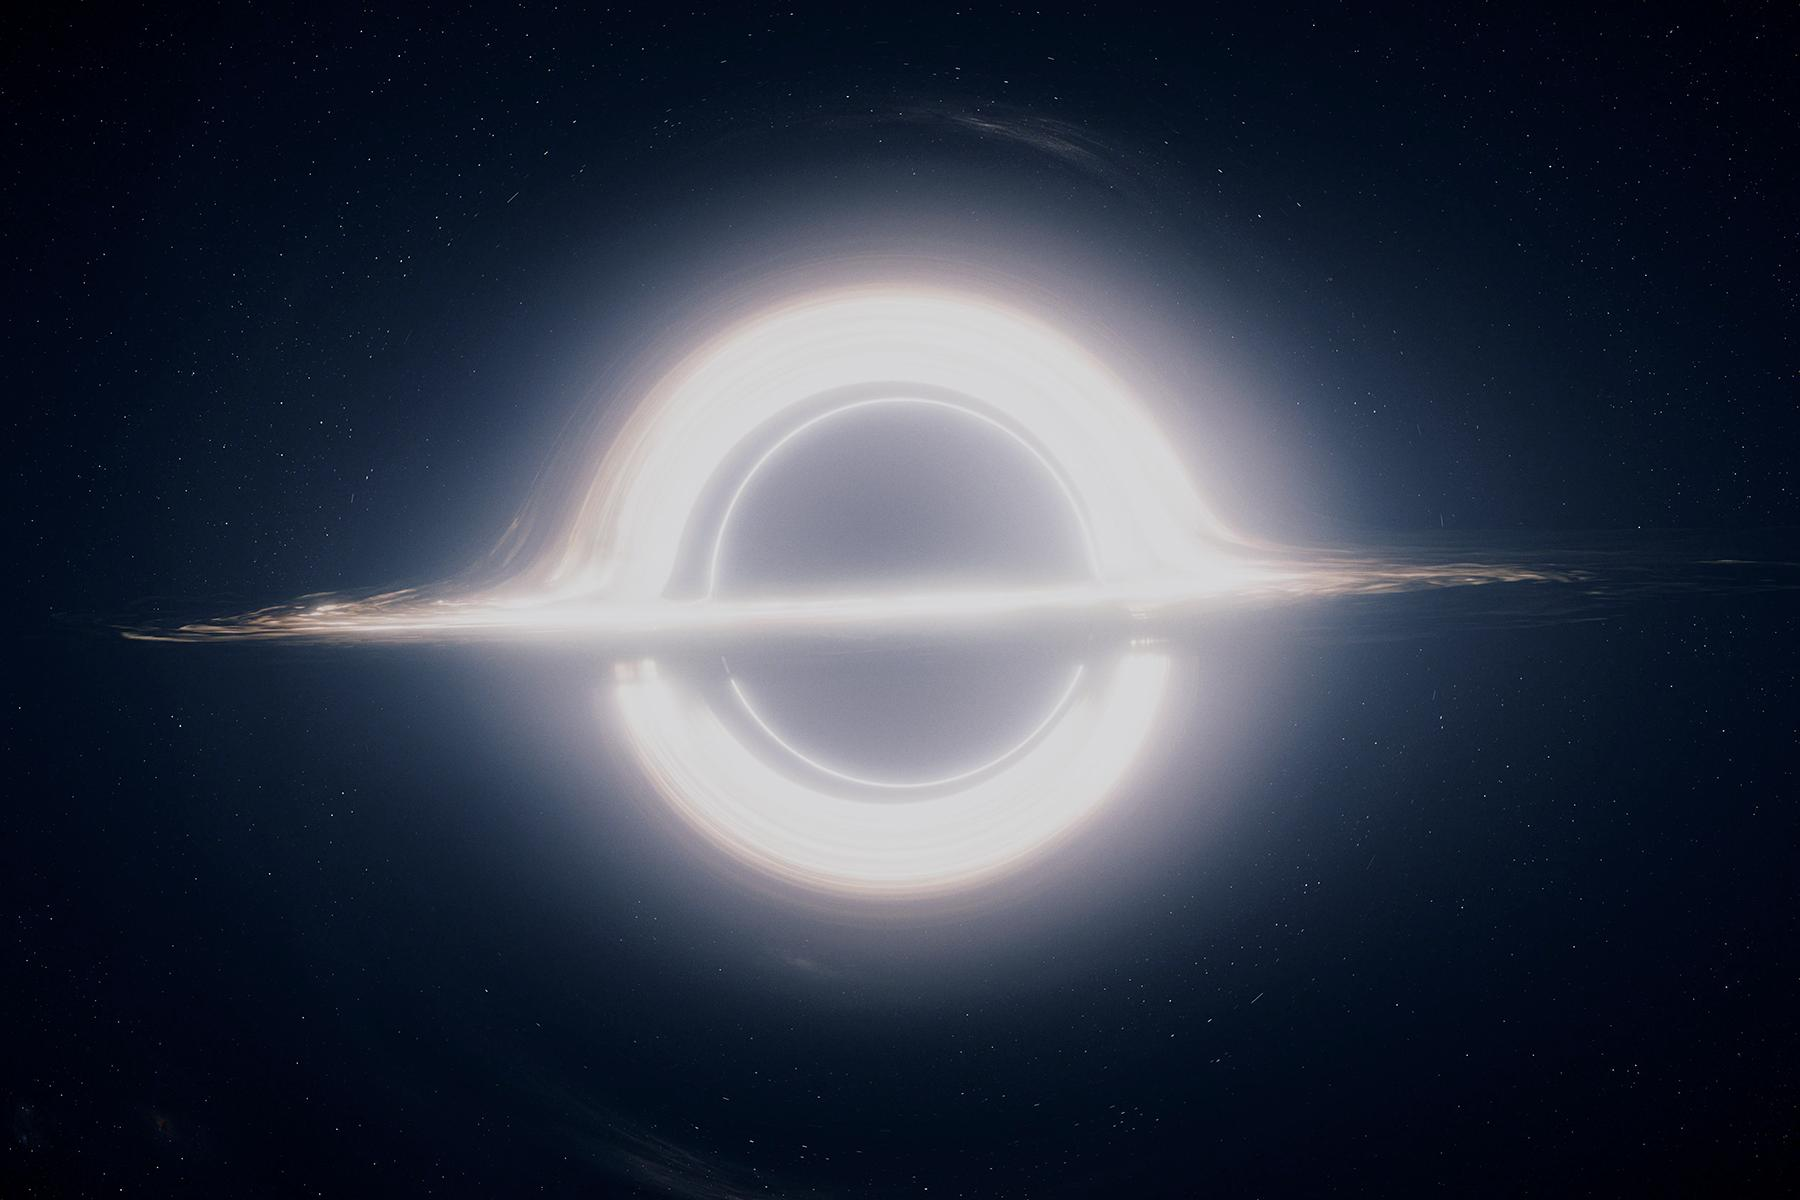
\includegraphics[scale=0.15]{images/gargantua.jpeg}
    \caption{Gargantua in \textit{Interstellar}}
    \label{fig:gargantua}
\end{figure}

My main focus for this project was to create programs to calculate how time dilates given a planet and a massive object
being orbited by it. To do this, I created classes in Python that represented a planet and another to represent stars, black
holes, and other massive objects in the universe.

\subsubsection{\texttt{Planet}}
The \texttt{Planet} class only needed to hold the name of the planet for reference, and its distance to its object keeping it
in orbit. An example of how to use the \texttt{Planet} class would be:
\begin{pylisting}{earth.py}
from planets import planets
earth = Planet("Earth", 1)
print(earth)
\end{pylisting}

\noindent Running this Python file would give you an output of:
\begin{bashlisting}{}
$\mbox{\textdollar}$ python earth.py
name: Earth     r: 1.0 AU
\end{bashlisting}

\subsection{\texttt{MassiveObject}}

The \texttt{MassiveObject} class is very similar to \texttt{Planet} but instead holds just the mass of the object. A similar 
example to use the class would be
\begin{pylisting}{sun.py}
from planets import MassiveObject
sun = MassiveObject("Sun", 1)
print(sun)
\end{pylisting}
Running \texttt{sun.py} would yield:
\begin{bashlisting}{}
$\mbox{\textdollar}$ python sun.py
name: Sun       solar mass: 1.0
\end{bashlisting}

\subsection{SciPy}

To use constants such as $G$ and $c$, \texttt{SciPy} is a great library with lots of different constants. Programming with
different units can get difficult, but \texttt{SciPy} makes this process easier by holding constants in terms of meters,
or seconds depending on the context. As seen above, the distance from the Earth to the Sun is shown in astronomical units.
In the background, the math is actually done in meters, so \texttt{earth.r} is set to \texttt{1 * constants.au}. To use this
library, one would simply include the line:
\begin{pylisting}{}
from scipy import constants
\end{pylisting}

\subsection{Time dilation function}

\noindent With these two classes, users can now create their own Python files using \texttt{planets.py} and calculate the
time dilation given an observed absolute time. The time dilation function definition is defined as:
$$\texttt{time\_dilation(t: float, planet: Planet, massive\_body: MassiveObject) -> float}$$
with \texttt{t} being $\Delta t$ and the return value being $\Delta t'$ as seen earlier. The first program I created with these
two classes was a calculation to find the distance from Miller's planet to Gargantua, as there was nothing on-line stating
its data. Given that the movie states one hour on Miller's planet is 7 years on Earth, I created a loop that calculated the time
dilation given a time of 7 years, and ran it until it equaled one hour. Below is the following program:
\begin{pylisting}{miller.py}
from planets import Planet, MassiveObject
from time_dilation import time_dilation
from scipy import constants


def main():
    gargantua = MassiveObject("Gargantua", 100000000)

    # figure out distance between Miller and Gargantua
    r = (2 * constants.G * gargantua.mass / constants.c**2)
    event_horizon = r
    print("Gargantua's event horizon:", event_horizon / constants.au)
    miller_time = 0
    while miller_time < constants.hour:
        miller = Planet("Miller", r / constants.au)
        miller_time = time_dilation(constants.year * 7, miller, gargantua)
        r += 1

    print(gargantua)
    print(miller)
    print("Miller is", miller.r - event_horizon, "meters away from Gargantua")
    print("7 years on Earth is", miller_time / constants.hour, "hours on Miller's planet")


if __name__ == "__main__":
    main()
\end{pylisting}

\noindent The output of this program is:
\begin{bashlisting}{}
$\mbox{\textdollar}$ python miller.py
Gargantua's event horizon: 1.985632612114088 AU
name: Gargantua	solar mass: 100000000.0
name: Miller	r: 1.9856326126421704 AU
Miller is 79.0 meters away from Gargantua
7 years on Earth is 1.0000081413217279 hours on Miller's planet
\end{bashlisting}

\noindent As shown from the output, Miller's planet should be 79 meters away from Gargantua for the gravitational physics
to be accurate, which is very close!

\subsection{\texttt{System}}

Extending the \texttt{Planet} and \texttt{MassiveObject} classes is the \texttt{System} class which holds planets and one
massive object which the planets orbit, to create a program \texttt{time\_dilation.py} that takes in a file and allows the 
user to experiment with the time dilation factors in that solar system. The file must be of the form
\begin{bashlisting}{}
Massive_Object_Name Solar_Mass
P1_Name Distance_AU
P2_Name Distance_AU
...
Pn_Name Distance_AU
\end{bashlisting}
where the distances of $n$ planets are in astronomical units, and the mass of the massive object is solar masses.
The text file below is an example which represents our solar system:
\begin{bashlisting}{solar\_system.txt}
Sun 1
Mercury 0.39
Venus 0.72
Earth 1
Mars 1.52
Jupiter 5.2
Saturn 9.54
Uranus 19.2
Neptune 30.06
\end{bashlisting}

\section{Running the program}

Running the program is simple, one needs to simply include a system of planets orbiting a star in the command
\begin{bashlisting}{}
$\mbox{\textdollar}$ python time_dilation.py [-f file_name]
\end{bashlisting}
By running this program with the \texttt{solar\_system.txt} file, one could have the following output comparing Earth's time
difference to Uranus' for 100,000,000 seconds observed in a vacuum
\begin{bashlisting}{}
$\mbox{\textdollar}$ python time_dilation.py -f solar_system.txt
Massive Object:
	name: Sun	    solar mass: 1.0
Planets:
	name: Mercury   r: 0.39 AU
	name: Venus	    r: 0.72 AU
	name: Earth	    r: 1.0 AU
	name: Mars	    r: 1.52 AU
	name: Jupiter   r: 5.2 AU
	name: Saturn    r: 9.54 AU
	name: Uranus    r: 19.2 AU
	name: Neptune   r: 30.06 AU

Enter two planets to calculate time dilation difference:
Planet 1: Uranus
Planet 2: Earth
Enter time observed in seconds: 100000000
Time on Uranus: 99999999.94829082
Time on Earth: 99999999.00718369
Time difference: 0.9411071389913559

Press ctrl-c to exit

Enter two planets to calculate time dilation difference:
Planet 1: ^C
$\mbox{\textdollar}$
\end{bashlisting}

\section{Conclusion}

\setlength{\epigraphwidth}{0.75\textwidth}
\epigraph{\emph{Two things are infinite: the universe and human stupidity; and I'm not sure about the universe.}}{--Albert Einstein}

Time dilation is just one very interesting concept that is a consequence of the special and general relativity theories developed by Albert Einstein,
but one that is mind-boggling when shown in a huge hypothetical setting such as Christopher Nolan's \textit{Interstellar} co-directed by Kip Thorne.
The GitHub repository at \href{https://github.com/ernaniraffo/time-dilation}{github.com/ernaniraffo/time-dilation} contains all the code of this project,
and can be used in a variety of ways. One could make their own hypothetical star or black-hole system such as in \textit{Interstellar}, and 
test different times to understand time dilation more.

\begin{figure}[h]
    \centering
    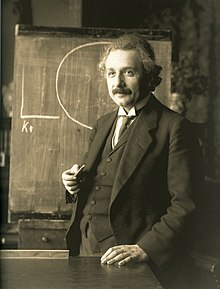
\includegraphics[scale=0.5]{images/einstein.jpg}
    \caption{Albert Einstein (1921)}
    \label{fig:einstein}
\end{figure}

\newpage
\centering In time's embrace, a love-hate affair, \\
Dilation's grip, both cruel and fair. \\
Moments elongate, passions ignite, \\
A paradoxical dance, my heart takes flight. \\



\end{document}

